% Case-B rotational-stiffness comparison. The legend gives the achieved
% pose-based initial angular-offset range across the three stiffness settings.
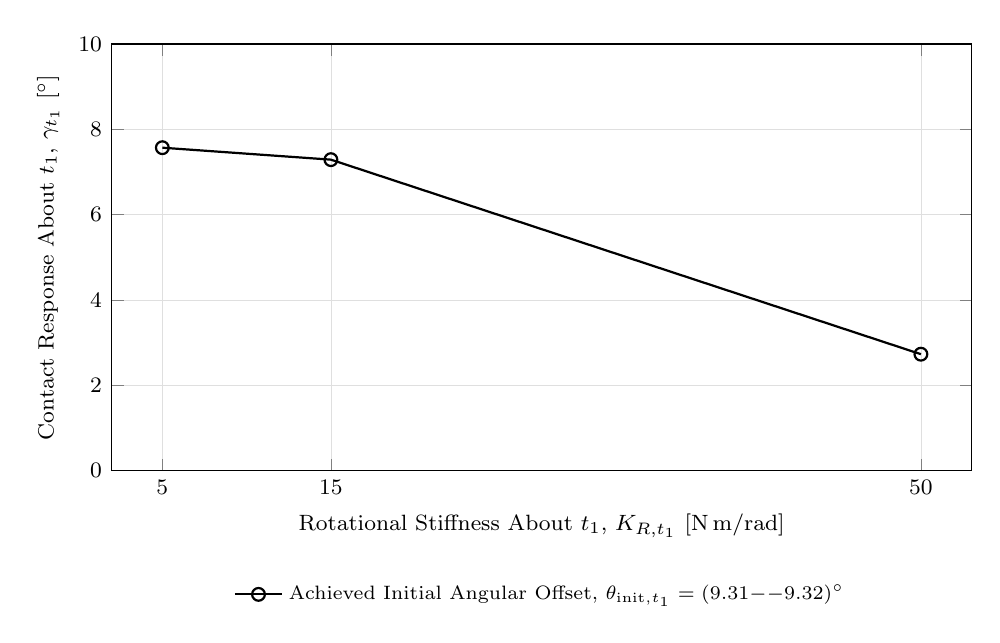
\begin{tikzpicture}
\begin{axis}[
    width=12.5cm, height=7.0cm,
    xmin=2, xmax=53, ymin=0, ymax=10,
    xtick={5,15,50},
    ytick={0,2,4,6,8,10},
    grid=major,
    grid style={gray!25, very thin},
    tick label style={font=\footnotesize},
    label style={font=\footnotesize},
    xlabel={Rotational Stiffness About \(t_1\), \(K_{R,t_1}\) [N\,m/rad]},
    ylabel={Contact Response About \(t_1\), \(\gamma_{t_1}\) [\(^\circ\)]},
    legend style={font=\scriptsize, draw=none, fill=none,
                  cells={anchor=west}, at={(0.5,-0.24)}, anchor=north},
    every axis plot/.append style={thick, mark size=2.3pt},
  ]
\addplot[black, mark=o] coordinates {
  (5,7.57) (15,7.29) (50,2.73)};
\addlegendentry{Achieved Initial Angular Offset, \(\theta_{\mathrm{init},t_1}=(9.31\text{--}9.32)^\circ\)}
\end{axis}
\end{tikzpicture}
